\documentclass{mwart} % Polska wersja klasy article

\usepackage{polski} % Pozwala na użycie polskiego. Ustawia między innymi fontenc na T1
\usepackage[utf8]{inputenc} % Informuje o kodowaniu
\usepackage{textcomp} % Znaki specjalne takie jak ~
\usepackage{xcolor} % Definicje kolorów

\renewcommand{\labelitemi}{\textbullet} % Zmiana symbolu wliczeń

\usepackage{graphicx}
\graphicspath{ {./Diagramy/} }
\usepackage{float} % Pozycjonowanie figur
\usepackage{mwe} % Tymczasowe grafiki

\usepackage{listings} % Listingi kodu
\lstset{basicstyle=\ttfamily,
  showstringspaces=false,
  commentstyle=\color{gray},
  keywordstyle=\color{blue}
}

\title{Laboratorium sieci komputerowych - c3 \\ Tworzenie i badanie sieci wewnętrznych}
\author{Krzysztof Dąbrowski gr. 3}
\date{\today}

\begin{document}
\maketitle{}
\tableofcontents{}
%\newpage

\section{Cel zajęć}
Celem laboratoriów \textit{c3} było utworzenie kilku sieci wewnętrznych oraz podłączenie do nich interfejsów maszyn wirtualnych. W celu nadania adresów wykorzystane zostało adresowanie statyczne oraz dynamiczne. Po zakończeniu konfiguracji sieci należało przeprowadzić analizę ruchu sieciowego.

\section{Schemat sieci}
Do wykonania zadań została utworzona sieć o schemacie przedstawionym poniżej.

%TODO: Schemat sieci
\begin{figure}[H]
  \centering
  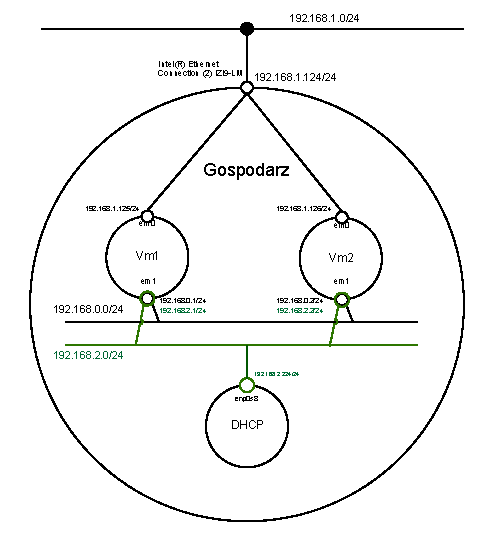
\includegraphics[width=\textwidth]{Projekt_Sieci}
  
  \caption{Schemat budowanej sieci}
  \label{fig:SchematSieci}
\end{figure}

\section{Statyczne adresowanie}
Ręcznie wybiorę adresy, które przypiszę statycznie interfejsom maszyn.

\subsection{Wybór adresów}
Ponieważ wiem, że będę potrzebował 2 sieci postanowiłem wykorzystać podsieci prywatnej sieci \texttt{192.168.0.0}. W celu ułatwienia obliczeń zdecydowałem, że maska podsieci będzie \textbf{24 bitowa}.

\begin{itemize}
  \item Adres pierwszej sieci -- \texttt{192.168.0.0/24}.
  \item Adres drugiej sieci -- \texttt{192.168.2.0/24}.
\end{itemize}

Maszyna BSD otrzyma statyczny adres \texttt{192.168.0.1/24}, maszyna Windows \texttt{192.168.0.2/24}, a maszyna Ubuntu adres \texttt{192.168.0.254/24}.

\subsection{Ustawienie adresów}
\subsubsection{Maszyna BSD}
Poleceniem \texttt{ifconfig} sprawdziłem, który interfejs jest podłączony do sieci wewnętrznej. Interfejs \texttt{em0} ma ustawiony adres ip, a \texttt{em1} nie ma. Dzięki temu wiem, że \textbf{em1} jest podłączony do sieci wewnętrznej.

Poleceniem \texttt{ifconfig em1 192.168.0.1/24} nadałem adres. By upewnić się, że polecenie zadziało wywołałem \texttt{ifconfig em1}.

\begin{verbatim}
root@:~ # ifconfig em1
em1: flags=8843<UP,BROADCAST,RUNNING,SIMPLEX,MULTICAST> metric 0 mtu 1500
        options=81009b<RXCSUM,TXCSUM,VLAN_MTU,VLAN_HWTAGGING,VLAN_HWCSUM,VLAN_HWFILTER>
        ether 08:00:27:d1:f2:36
        inet 192.168.0.1 netmask 0xffffff00 broadcast 192.168.0.255
        media: Ethernet autoselect (1000baseT <full-duplex>)
        status: active
        nd6 options=29<PERFORMNUD,IFDISABLED,AUTO_LINKLOCAL>
\end{verbatim}

\subsubsection{Maszyna Ubuntu}
Poleceniem \texttt{ifconfig} sprawdziłem, który interfejs jest podłączony do sieci wewnętrznej. Interfejs \texttt{enp0s3} ma ustawiony adres ip, a \texttt{enp0s8} nie ma. Dzięki temu wiem, że \textbf{enp0s8} jest podłączony do sieci wewnętrznej.

Poleceniem \texttt{sudo ip address add 192.168.0.254/24 dev enp0s8} nadałem adres. By upewnić się, że polecenie zadziało wywołałem \texttt{ip a}.

\begin{verbatim}
3: enp0s8: <BROADCAST,MULTICAST,UP,LOWER_UP> mtu 1500 qdisc pfifo_fast state UP group default qlen 1000
link/ether 08:00:27:c2:b7:2e brd ff:ff:ff:ff:ff:ff
inet 192.168.0.254/24 scope global enp0s8
        valid_lft forever preferred_lft forever
inet6 fe80::a00:27ff:fec2:b72e/64 scope link
        valid_lft forever preferred_lft forever
\end{verbatim}

\subsubsection{Maszyna Windows}
Poleceniem \texttt{ipconfig} sprawdziłem, który interfejs jest podłączony do sieci wewnętrznej. Interfejs \texttt{Ethernet} ma ustawiony adres ip, a \texttt{Ethernet 2} nie ma. Dzięki temu wiem, że \textbf{Ethernet 2} jest podłączony do sieci wewnętrznej.

Poleceniem \texttt{netsh interface ip set address "Ethernet 2" static 192.168.0.2 255.255.255.0} nadałem adres. By upewnić się, że polecenie zadziało wywołałem \texttt{ipconfig}.

\begin{verbatim}
Ethernet adapter Ethernet 2:

        Connection-specific DNS Suffix  . :
        Link-local IPv6 Address . . . . . : fe80::84c8:23f5:a0ee:874e%2
        IPv4 Address. . . . . . . . . . . : 192.168.0.2
        Subnet Mask . . . . . . . . . . . : 255.255.255.0
        Default Gateway . . . . . . . . . :  
\end{verbatim}

\subsection{Test połączenia}
W celu sprawdzenia utworzonej konfiguracji wysłałem ping między maszynami. Będąc zalogowanym na Ubuntu wykonałem \texttt{ping 192.168.0.1 -c 1},

\begin{verbatim}
PING 192.168.0.1 (192.168.0.1) 56(84) bytes of data. 
64 bytes from 192.168.0.1: icmp_seq=1 ttl=64 time=0.379 ms

--- 192.168.0.1 ping statistics ---
1 packets transmitted, 1 received, 0% packet loss, time 0ms
rtt min/avg/max/mdev = 0.379/0.379/0.379/0.000 ms
\end{verbatim}

Oraz \texttt{ping 192.168.0.254 -c }.

\begin{verbatim}
PING 192.168.0.254 (192.168.0.254) 56(84) bytes of data. 
64 bytes from 192.168.0.254: icmp_seq=1 ttl=64 time=0.019 ms

--- 192.168.0.254 ping statistics ---
1 packets transmitted, 1 received, 0% packet loss, time 0ms
rtt min/avg/max/mdev = 0.019/0.019/0.019/0.000 ms
\end{verbatim}

Z wyniku komend widać, że maszyny są ze sobą połączone i mogą wymieniać informacje.

\section{Dynamiczne adresowanie}
Postanowiłem wykorzystać maszynę Ubuntu jako serwer DHCP. Położyłem statycznie adres z drugiej sieci poleceniem \texttt{sudo ip a add 192.168.2.254 dev enp0s8}.

\subsection{Konfiguracja serwera}
Zainstalowałem serwer DHCP poleceniem \texttt{sudo apt install isc-dhcp-server}. Następnie skonfigurowałem serwer edytując dwa pliki systemowe.

W pliku \texttt{/etc/default/isc-dhcp-server} umieściłem linię \texttt{INTERFACES="enp0s8"}, która wskazuje na jakim interfejsie serwer DHCP ma pracować.

W pliku \texttt{/etc/dhcp/dhcpd.conf} umieściłem konfigurację samego serwera. Zawartość tego pliku wygląda następująco:

\begin{verbatim}
ddns-update-style none;
default-lease-time 600;
max-lease-time 7200;

subnet 192.168.2.0 netmask 255.255.255.0 {
  range 192.168.2.1 192.168.2.253;
}
\end{verbatim}

Definiuje on na jaki czas będą przydzielane adresy oraz z jakie puli będą pochodzić.

Po zakończeniu konfiguracji uruchomiłem serwer poleceniem \texttt{sudo systemctl start isc-dhcp-server.service} oraz \texttt{sudo systemctl enable isc-dhcp-server.service}

\vspace{3mm}
By sprawdzić czy serwer działa wykonałem komendę \texttt{systemctl status isc-dhcp-server.service}.
\begin{verbatim}
  isc-dhcp-server.service - ISC DHCP IPv4 server
   Loaded: loaded (/lib/systemd/system/isc-dhcp-server.service; enabled; vendor preset: enabled)
   Active: active (running) since wto 2019-04-16 18:06:48 CEST; 14min ago
     Docs: man:dhcpd(8)
 Main PID: 3186 (dhcpd)
   CGroup: /system.slice/isc-dhcp-server.service
           3186 dhcpd -user dhcpd -group dhcpd -f -4 -pf /run/dhcp-server/dhcpd.pid -cf /etc/dhcp/dhcpd.conf enp0s8
\end{verbatim}

\subsection{Dynamiczne przydzielenie adresów}

\subsubsection{Maszyna BSD}
By pozyskać adres od serwera DHCP na maszynie BSD uruchomiłem komendę \texttt{dhclient em1}.

\vspace{2mm}
\begin{verbatim}
DHCPDISCOVER on em1 to 255.255.255.255 port 67 interval 7 
DHCPOFFER from 192.168.2.254 
DHCPREQUEST on em1 to 255.255.255.255 port 67 
DHCPACK from 192.168.2.254 
bound to 192.168.2.1 -- renewal in 300 seconds.
\end{verbatim}

\subsubsection{Maszyna Windows}
By móc pozyskać adres od serwera DHCP ustawiłem dynamiczne pobieranie adresów poleceniem \texttt{netsh interface ip set address "Ethernet 2" dhcp}.

By sprawdzić wynik uruchomiłem \texttt{ipconfig}.
\begin{verbatim}
Ethernet adapter Ethernet 2:

        Connection-specific DNS Suffix  . :
        Link-local IPv6 Address . . . . . : fe80::84c8:23f5:a0ee:874e%2
        IPv4 Address. . . . . . . . . . . : 192.168.2.3
        Subnet Mask . . . . . . . . . . . : 255.255.255.0
        Default Gateway . . . . . . . . . : 
\end{verbatim}

Widać, że interfejs \texttt{Ethernet 2} otrzymał dynamicznie adres z puli adresów serwera DHCP.
 
\section{Druga warstwa sieciowa}
Od początku planowałem kładzenie drugiej warstwy sieciowej. Skonfigurowałem serwer DHCP w ten sposób, że przydziela on adresy z drugiej, oddzielnej sieci niż adresy ustawione statycznie. Można to łatwo sprawdzić listując interfejsy maszyn.

\paragraph{BSD:}
\begin{verbatim}
root@:~ # ifconfig  
em0: flags=8843<UP,BROADCAST,RUNNING,SIMPLEX,MULTICAST> metric 0 mtu 1500 
        options=81009b<RXCSUM,TXCSUM,VLAN_MTU,VLAN_HWTAGGING,VLAN_HWCSUM,VLAN_HWFILTER>
        ether 08:00:27:a7:2f:18
        inet 192.168.1.128 netmask 0xffffff00 broadcast 192.168.1.255
        media: Ethernet autoselect (1000baseT <full-duplex>)
        status: active
        nd6 options=29<PERFORMNUD,IFDISABLED,AUTO_LINKLOCAL>
em1: flags=8843<UP,BROADCAST,RUNNING,SIMPLEX,MULTICAST> metric 0 mtu 1500
        options=81009b<RXCSUM,TXCSUM,VLAN_MTU,VLAN_HWTAGGING,VLAN_HWCSUM,VLAN_HWFILTER>
        ether 08:00:27:d1:f2:36
        inet 192.168.0.1 netmask 0xffffff00 broadcast 192.168.0.255
        inet 192.168.2.1 netmask 0xffffff00 broadcast 192.168.2.255
        media: Ethernet autoselect (1000baseT <full-duplex>)
        status: active
        nd6 options=29<PERFORMNUD,IFDISABLED,AUTO_LINKLOCAL>
lo0: flags=8049<UP,LOOPBACK,RUNNING,MULTICAST> metric 0 mtu 16384
        options=680003<RXCSUM,TXCSUM,LINKSTATE,RXCSUM_IPV6,TXCSUM_IPV6>
        inet6 ::1 prefixlen 128
        inet6 fe80::1%lo0 prefixlen 64 scopeid 0x3
        inet 127.0.0.1 netmask 0xff000000
        groups: lo
        nd6 options=21<PERFORMNUD,AUTO_LINKLOCAL>
\end{verbatim}

\paragraph{Ubuntu:}
\begin{verbatim}
root@:~ # ifconfig  
em0: flags=8843<UP,BROADCAST,RUNNING,SIMPLEX,MULTICAST> metric 0 mtu 1500 
        options=81009b<RXCSUM,TXCSUM,VLAN_MTU,VLAN_HWTAGGING,VLAN_HWCSUM,VLAN_HWFILTER>
        ether 08:00:27:a7:2f:18
        inet 192.168.1.128 netmask 0xffffff00 broadcast 192.168.1.255
        media: Ethernet autoselect (1000baseT <full-duplex>)
        status: active
        nd6 options=29<PERFORMNUD,IFDISABLED,AUTO_LINKLOCAL>
em1: flags=8843<UP,BROADCAST,RUNNING,SIMPLEX,MULTICAST> metric 0 mtu 1500
        options=81009b<RXCSUM,TXCSUM,VLAN_MTU,VLAN_HWTAGGING,VLAN_HWCSUM,VLAN_HWFILTER>
        ether 08:00:27:d1:f2:36
        inet 192.168.0.1 netmask 0xffffff00 broadcast 192.168.0.255
        inet 192.168.2.1 netmask 0xffffff00 broadcast 192.168.2.255
        media: Ethernet autoselect (1000baseT <full-duplex>)
        status: active
        nd6 options=29<PERFORMNUD,IFDISABLED,AUTO_LINKLOCAL>
lo0: flags=8049<UP,LOOPBACK,RUNNING,MULTICAST> metric 0 mtu 16384
        options=680003<RXCSUM,TXCSUM,LINKSTATE,RXCSUM_IPV6,TXCSUM_IPV6>
        inet6 ::1 prefixlen 128
        inet6 fe80::1%lo0 prefixlen 64 scopeid 0x3
        inet 127.0.0.1 netmask 0xff000000
        groups: lo
        nd6 options=21<PERFORMNUD,AUTO_LINKLOCAL>
\end{verbatim}

Widać wyraźnie, że interfejsy mają przypisane \textbf{dwa} adresy ip z różnych sieci.

\section{Analiza ruchu sieciowego}
W celu zbadania ruchu sieciowego skorzystam z konsolowego narzędzia \texttt{tcpdump}.

\subsection{Badanie ARP}
By przechwycić ruch związany z protokołem ARP uruchomiłem nasłuchiwanie na maszynie Ubuntu poleceniem \texttt{sudo tcpdump -i em1 -X arp}.

Maszyna BSD ma zapamiętany adres MAC maszyny Windows ponieważ wykonywałem pingowanie. Aby to zmienić muszę wyczyścić cashe ARP poleceniem \texttt{arp -d -a}.

Wykonałem polecenie \texttt{ping -c 1 192.168.2.254} na maszynie BSD by sprowokować użycie ARP.

\paragraph{Wynik działania tcpdump:}
\begin{verbatim}
# tcpdump -i em1 -X arp
tcpdump: verbose output suppressed, use -v or -vv for full protocol decode
listening on em1, link-type EN10MB (Ethernet), capture size 262144 bytes
20:01:54.524167 ARP, Request who-has 192.168.2.254 tell 192.168.2.1, length 46 
        0x0000:  0001 0800 0604 0001 0800 27d1 f236 c0a8  ..........'..6..
        0x0010:  0201 0000 0000 0000 c0a8 02fe 0000 0000  ................
        0x0020:  0000 0000 0000 0000 0000 0000 0000       ..............
^C
1 packet captured
1 packet received by filter
0 packets dropped by kernel
\end{verbatim}

Z przechwyconych informacji można wywnioskować, że maszyna o adresie \texttt{192.168.2.1} pytała o to kto ma adres \texttt{192.168.2.254}.

\subsection{Badanie DHCP}

\subsubsection{Maszyna BSD}
By przechwycić ruch związany z dynamicznym nadawaniem adresów uruchomiłem nasłuchiwanie na maszynie Ubuntu poleceniem \texttt{sudo tcpdump -i enp0s8 port 67 or port 68 -X}.

By móc na nowo pozyskać adres na maszynie BSD zatrzymałem działającego klienta DHCP poleceniem \texttt{kill -9 931}. Następnie wywołałem \texttt{dhclient em1}. Zwrócony został następujący komunikat.
\begin{verbatim}
DHCPREQUEST on em1 to 255.255.255.255 port 67 
DHCPACK from 192.168.2.254 
bound to 192.168.2.1 -- renewal in 300 seconds.
\end{verbatim}

\paragraph{Wynik działania tcpdump:}
\begin{footnotesize}
\begin{verbatim}
tcpdump: verbose output suppressed, use -v or -vv for full protocol decode 
listening on enp0s8, link-type EN10MB (Ethernet), capture size 262144 bytes
20:06:47.429724 IP 0.0.0.0.bootpc > 255.255.255.255.bootps: BOOTP/DHCP, Request from 08:00:27:d1:f2:36 (oui Unknown), length 300 
        0x0000:  4510 0148 0000 0000 8011 3996 0000 0000  E..H......9.....
        0x0010:  ffff ffff 0044 0043 0134 095f 0101 0600  .....D.C.4._....
        0x0020:  0ca1 3dff 0000 0000 0000 0000 0000 0000  ..=.............
        0x0030:  0000 0000 0000 0000 0800 27d1 f236 0000  ..........'..6..
        0x0040:  0000 0000 0000 0000 0000 0000 0000 0000  ................
        0x0050:  0000 0000 0000 0000 0000 0000 0000 0000  ................
        0x0060:  0000 0000 0000 0000 0000 0000 0000 0000  ................
        0x0070:  0000 0000 0000 0000 0000 0000 0000 0000  ................
        0x0080:  0000 0000 0000 0000 0000 0000 0000 0000  ................
        0x0090:  0000 0000 0000 0000 0000 0000 0000 0000  ................
        0x00a0:  0000 0000 0000 0000 0000 0000 0000 0000  ................
        0x00b0:  0000 0000 0000 0000 0000 0000 0000 0000  ................
        0x00c0:  0000 0000 0000 0000 0000 0000 0000 0000  ................
        0x00d0:  0000 0000 0000 0000 0000 0000 0000 0000  ................
        0x00e0:  0000 0000 0000 0000 0000 0000 0000 0000  ................
        0x00f0:  0000 0000 0000 0000 0000 0000 0000 0000  ................
        0x0100:  0000 0000 0000 0000 6382 5363 3501 0332  ........c.Sc5..2
        0x0110:  04c0 a802 013d 0701 0800 27d1 f236 370a  .....=....'..67.
        0x0120:  011c 0279 030f 060c 771a ff00 0000 0000  ...y....w.......
        0x0130:  0000 0000 0000 0000 0000 0000 0000 0000  ................
        0x0140:  0000 0000 0000 0000                      ........
20:06:47.441442 IP 192.168.2.254.bootps > 192.168.2.1.bootpc: BOOTP/DHCP, Reply, length 300 
        0x0000:  4510 0148 0000 0000 8011 b345 c0a8 02fe  E..H.......E....
        0x0010:  c0a8 0201 0043 0044 0134 7da0 0201 0600  .....C.D.4}.....
        0x0020:  0ca1 3dff 0000 0000 0000 0000 c0a8 0201  ..=.............
        0x0030:  c0a8 02fe 0000 0000 0800 27d1 f236 0000  ..........'..6..
        0x0040:  0000 0000 0000 0000 0000 0000 0000 0000  ................
        0x0050:  0000 0000 0000 0000 0000 0000 0000 0000  ................
        0x0060:  0000 0000 0000 0000 0000 0000 0000 0000  ................
        0x0070:  0000 0000 0000 0000 0000 0000 0000 0000  ................
        0x0080:  0000 0000 0000 0000 0000 0000 0000 0000  ................
        0x0090:  0000 0000 0000 0000 0000 0000 0000 0000  ................
        0x00a0:  0000 0000 0000 0000 0000 0000 0000 0000  ................
        0x00b0:  0000 0000 0000 0000 0000 0000 0000 0000  ................
        0x00c0:  0000 0000 0000 0000 0000 0000 0000 0000  ................
        0x00d0:  0000 0000 0000 0000 0000 0000 0000 0000  ................
        0x00e0:  0000 0000 0000 0000 0000 0000 0000 0000  ................
        0x00f0:  0000 0000 0000 0000 0000 0000 0000 0000  ................
        0x0100:  0000 0000 0000 0000 6382 5363 3501 0536  ........c.Sc5..6
        0x0110:  04c0 a802 fe33 0400 0002 5801 04ff ffff  .....3....X.....
        0x0120:  00ff 0000 0000 0000 0000 0000 0000 0000  ................
        0x0130:  0000 0000 0000 0000 0000 0000 0000 0000  ................
        0x0140:  0000 0000 0000 0000                      ........
^C 
2 packets captured
2 packets received by filter
0 packets dropped by kernel
\end{verbatim}
\end{footnotesize}

\subsubsection{Maszyna Windows}
By przechwycić ruch związany z dynamicznym nadawaniem adresów uruchomiłem nasłuchiwanie na maszynie Ubuntu poleceniem \texttt{sudo tcpdump -i enp0s8 port 67 or port 68 -X}.

W celu pozbycia się wcześniej uzyskanego adresu wpisałem komendę \texttt{ipconfig /release}.
Następnie by pozyskać adres od serwera DHCP wpisałem \texttt{ipconfig /renew}

\paragraph{Wynik działania tcpdump:}
\begin{footnotesize}
\begin{verbatim}
tcpdump: verbose output suppressed, use -v or -vv for full protocol decode 
listening on enp0s8, link-type EN10MB (Ethernet), capture size 262144 bytes
20:06:47.429724 IP 0.0.0.0.bootpc > 255.255.255.255.bootps: BOOTP/DHCP, Request from 08:00:27:d1:f2:36 (oui Unknown), length 300 
        0x0000:  4510 0148 0000 0000 8011 3996 0000 0000  E..H......9.....
        0x0010:  ffff ffff 0044 0043 0134 095f 0101 0600  .....D.C.4._....
        0x0020:  0ca1 3dff 0000 0000 0000 0000 0000 0000  ..=.............
        0x0030:  0000 0000 0000 0000 0800 27d1 f236 0000  ..........'..6..
        0x0040:  0000 0000 0000 0000 0000 0000 0000 0000  ................
        0x0050:  0000 0000 0000 0000 0000 0000 0000 0000  ................
        0x0060:  0000 0000 0000 0000 0000 0000 0000 0000  ................
        0x0070:  0000 0000 0000 0000 0000 0000 0000 0000  ................
        0x0080:  0000 0000 0000 0000 0000 0000 0000 0000  ................
        0x0090:  0000 0000 0000 0000 0000 0000 0000 0000  ................
        0x00a0:  0000 0000 0000 0000 0000 0000 0000 0000  ................
        0x00b0:  0000 0000 0000 0000 0000 0000 0000 0000  ................
        0x00c0:  0000 0000 0000 0000 0000 0000 0000 0000  ................
->  ~ sudo tcpdump -i enp0s8 port 67 or port 68 -X 
tcpdump: verbose output suppressed, use -v or -vv for full protocol decode  
listening on enp0s8, link-type EN10MB (Ethernet), capture size 262144 bytes 
20:11:41.195971 IP 0.0.0.0.bootpc > 255.255.255.255.bootps: BOOTP/DHCP, Request from 08:00:27:07:df:cb (oui Unknown), length 302 
        0x0000:  4500 014a 4280 0000 8011 f723 0000 0000  E..JB......#....
        0x0010:  ffff ffff 0044 0043 0136 769f 0101 0600  .....D.C.6v.....
        0x0020:  efc1 01d4 0000 0000 0000 0000 0000 0000  ................
        0x0030:  0000 0000 0000 0000 0800 2707 dfcb 0000  ..........'.....
        0x0040:  0000 0000 0000 0000 0000 0000 0000 0000  ................
        0x0050:  0000 0000 0000 0000 0000 0000 0000 0000  ................
        0x0060:  0000 0000 0000 0000 0000 0000 0000 0000  ................
        0x0070:  0000 0000 0000 0000 0000 0000 0000 0000  ................
        0x0080:  0000 0000 0000 0000 0000 0000 0000 0000  ................
        0x0090:  0000 0000 0000 0000 0000 0000 0000 0000  ................
        0x00a0:  0000 0000 0000 0000 0000 0000 0000 0000  ................
        0x00b0:  0000 0000 0000 0000 0000 0000 0000 0000  ................
        0x00c0:  0000 0000 0000 0000 0000 0000 0000 0000  ................
        0x00d0:  0000 0000 0000 0000 0000 0000 0000 0000  ................
        0x00e0:  0000 0000 0000 0000 0000 0000 0000 0000  ................
        0x00f0:  0000 0000 0000 0000 0000 0000 0000 0000  ................
        0x0100:  0000 0000 0000 0000 6382 5363 3501 013d  ........c.Sc5..=
        0x0110:  0701 0800 2707 dfcb 3204 c0a8 0203 0c0f  ....'...2.......
        0x0120:  4445 534b 544f 502d 4c52 5352 4144 353c  DESKTOP-LRSRAD5<
        0x0130:  084d 5346 5420 352e 3037 0e01 0306 0f1f  .MSFT.5.07......
        0x0140:  212b 2c2e 2f77 79f9 fcff                 !+,./wy...
20:11:42.198007 IP 192.168.2.254.bootps > 192.168.2.3.bootpc: BOOTP/DHCP, Reply, length 300 
        0x0000:  4510 0148 0000 0000 8011 b343 c0a8 02fe  E..H.......C....
        0x0010:  c0a8 0203 0043 0044 0134 ecdb 0201 0600  .....C.D.4......
        0x0020:  efc1 01d4 0000 0000 0000 0000 c0a8 0203  ................
        0x0030:  c0a8 02fe 0000 0000 0800 2707 dfcb 0000  ..........'.....
        0x0040:  0000 0000 0000 0000 0000 0000 0000 0000  ................
        0x0050:  0000 0000 0000 0000 0000 0000 0000 0000  ................
        0x0060:  0000 0000 0000 0000 0000 0000 0000 0000  ................
        0x0070:  0000 0000 0000 0000 0000 0000 0000 0000  ................
        0x0080:  0000 0000 0000 0000 0000 0000 0000 0000  ................
        0x0090:  0000 0000 0000 0000 0000 0000 0000 0000  ................
        0x00a0:  0000 0000 0000 0000 0000 0000 0000 0000  ................
        0x00b0:  0000 0000 0000 0000 0000 0000 0000 0000  ................
        0x00c0:  0000 0000 0000 0000 0000 0000 0000 0000  ................
        0x00d0:  0000 0000 0000 0000 0000 0000 0000 0000  ................
        0x00e0:  0000 0000 0000 0000 0000 0000 0000 0000  ................
        0x00f0:  0000 0000 0000 0000 0000 0000 0000 0000  ................
        0x0100:  0000 0000 0000 0000 6382 5363 3501 0236  ........c.Sc5..6
        0x0110:  04c0 a802 fe33 0400 0002 5801 04ff ffff  .....3....X.....
        0x0120:  00ff 0000 0000 0000 0000 0000 0000 0000  ................
        0x0130:  0000 0000 0000 0000 0000 0000 0000 0000  ................
        0x0140:  0000 0000 0000 0000                      ........
20:11:42.199351 IP 0.0.0.0.bootpc > 255.255.255.255.bootps: BOOTP/DHCP, Request from 08:00:27:07:df:cb (oui Unknown), length 328       
        0x0000:  4500 0164 4281 0000 8011 f708 0000 0000  E..dB...........
        0x0010:  ffff ffff 0044 0043 0150 1679 0101 0600  .....D.C.P.y....
        0x0020:  efc1 01d4 0000 0000 0000 0000 0000 0000  ................
        0x0030:  0000 0000 0000 0000 0800 2707 dfcb 0000  ..........'.....
        0x0040:  0000 0000 0000 0000 0000 0000 0000 0000  ................
        0x0050:  0000 0000 0000 0000 0000 0000 0000 0000  ................
        0x0060:  0000 0000 0000 0000 0000 0000 0000 0000  ................
        0x0070:  0000 0000 0000 0000 0000 0000 0000 0000  ................
        0x0080:  0000 0000 0000 0000 0000 0000 0000 0000  ................
        0x0090:  0000 0000 0000 0000 0000 0000 0000 0000  ................
        0x00a0:  0000 0000 0000 0000 0000 0000 0000 0000  ................
        0x00b0:  0000 0000 0000 0000 0000 0000 0000 0000  ................
        0x00c0:  0000 0000 0000 0000 0000 0000 0000 0000  ................
        0x00d0:  0000 0000 0000 0000 0000 0000 0000 0000  ................
        0x00e0:  0000 0000 0000 0000 0000 0000 0000 0000  ................
        0x00f0:  0000 0000 0000 0000 0000 0000 0000 0000  ................
        0x0100:  0000 0000 0000 0000 6382 5363 3501 033d  ........c.Sc5..=
        0x0110:  0701 0800 2707 dfcb 3204 c0a8 0203 3604  ....'...2.....6.
        0x0120:  c0a8 02fe 0c0f 4445 534b 544f 502d 4c52  ......DESKTOP-LR
        0x0130:  5352 4144 3551 1200 0000 4445 534b 544f  SRAD5Q....DESKTO
        0x0140:  502d 4c52 5352 4144 353c 084d 5346 5420  P-LRSRAD5<.MSFT.
        0x0150:  352e 3037 0e01 0306 0f1f 212b 2c2e 2f77  5.07......!+,./w
        0x0160:  79f9 fcff                                y...
20:11:42.213375 IP 192.168.2.254.bootps > 192.168.2.3.bootpc: BOOTP/DHCP, Reply, length 300
        0x0000:  4510 0148 0000 0000 8011 b343 c0a8 02fe  E..H.......C....
        0x0010:  c0a8 0203 0043 0044 0134 e9db 0201 0600  .....C.D.4......
        0x0020:  efc1 01d4 0000 0000 0000 0000 c0a8 0203  ................
        0x0030:  c0a8 02fe 0000 0000 0800 2707 dfcb 0000  ..........'.....
        0x0040:  0000 0000 0000 0000 0000 0000 0000 0000  ................
        0x0050:  0000 0000 0000 0000 0000 0000 0000 0000  ................
        0x0060:  0000 0000 0000 0000 0000 0000 0000 0000  ................
        0x0070:  0000 0000 0000 0000 0000 0000 0000 0000  ................
        0x0080:  0000 0000 0000 0000 0000 0000 0000 0000  ................
        0x0090:  0000 0000 0000 0000 0000 0000 0000 0000  ................
        0x00a0:  0000 0000 0000 0000 0000 0000 0000 0000  ................
        0x00b0:  0000 0000 0000 0000 0000 0000 0000 0000  ................ 
        0x00c0:  0000 0000 0000 0000 0000 0000 0000 0000  ................
        0x00d0:  0000 0000 0000 0000 0000 0000 0000 0000  ................
        0x00e0:  0000 0000 0000 0000 0000 0000 0000 0000  ................
        0x00f0:  0000 0000 0000 0000 0000 0000 0000 0000  ................
        0x0100:  0000 0000 0000 0000 6382 5363 3501 0536  ........c.Sc5..6
        0x0110:  04c0 a802 fe33 0400 0002 5801 04ff ffff  .....3....X.....
        0x0120:  00ff 0000 0000 0000 0000 0000 0000 0000  ................
        0x0130:  0000 0000 0000 0000 0000 0000 0000 0000  ................
        0x0140:  0000 0000 0000 0000                      ........
^C 
4 packets captured
4 packets received by filter
0 packets dropped by kernel
\end{verbatim}
\end{footnotesize}
\end{document}